
\section{两个\trCriticalPoint{}之间的连接空间，或“\trBrokenTrajectory”空间}
\label{sec:space-of-connections}

\subsection{\trBrokenTrajectory{}的空间}
\label{subsec:space-broken-trajectories}

设 $a$ 与 $b$ 是 $f$ 的两个\trCriticalPoint，我们令 $\mathcal{L}(a,b)$ 表示\trVectorField{} $X$ 的那些从 $a$ 走到 $b$ 的\trTrajectory{}所成之集。我们把从 $a$ 到 $b$ 的\trBrokenTrajectory{}之集定义如下：
\[
\overline{\mathcal{L}}(a,b)=\bigcup_{c_i\in\operatorname{Crit}(f)}
  \mathcal{L}(a,c_1)\times\cdots\times\mathcal{L}(c_{q-1},b)\text{。}
\]
让我们回忆一下，\trIndex{}沿 $X$ 的诸\trTrajectory{}是递减的；因此，只有那些满足 $\operatorname{Ind}(c_i)>\operatorname{Ind}(c_{i+1})$ 的 $\mathcal{L}(c_i,c_{i+1})$ 才有贡献。

正如记号所提示的那样，这个空间意在成为 $\mathcal{L}(a,b)$ 的一个\trCompactification。要做的第一件事，就是赋予它一个\trTopology。这当然需要在这个并的每一项上诱导出乘积\trTopology。在\cref{fig:compactification-interval}所描述的例子里，$\mathcal{L}(a,b)$ 是一个\trOpen{}区间，而 $\mathcal{L}(a,c_1)$ 与 $\mathcal{L}(c_1,b)$ 都是点，$\mathcal{L}(a,c_2)$ 与 $\mathcal{L}(c_2,b)$ 亦然。我们当然希望赋予空间 $\overline{\mathcal{L}}(a,b)$ 一个使它成为闭区间的\trTopology。参见\cref{fig:union-intervals}。

\begin{figure}[htbp]
\centering
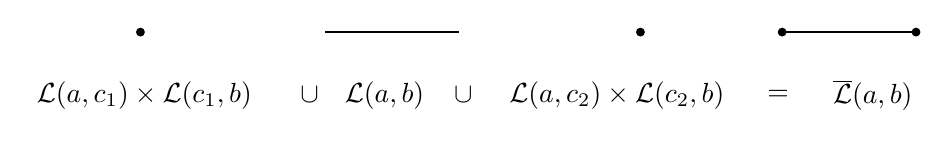
\begin{tikzpicture}[line width=0.6pt]
  \fill (0,1.05) circle (1.6pt);
  \draw (2.35,1.05) -- (4.05,1.05);
  \fill (6.35,1.05) circle (1.6pt);
  \draw (8.15,1.05) -- (9.85,1.05);
  \fill (8.15,1.05) circle (1.6pt);
  \fill (9.85,1.05) circle (1.6pt);
  \node at (0.05,0.25) {$\mathcal{L}(a,c_1)\times\mathcal{L}(c_1,b)$};
  \node at (2.15,0.25) {$\,\cup\,$};
  \node at (3.1,0.25) {$\mathcal{L}(a,b)$};
  \node at (4.1,0.25) {$\,\cup\,$};
  \node at (6.05,0.25) {$\mathcal{L}(a,c_2)\times\mathcal{L}(c_2,b)$};
  \node at (8.1,0.25) {$\,=\,$};
  \node at (9.3,0.25) {$\overline{\mathcal{L}}(a,b)$};
\end{tikzpicture}
\caption{}
\label{fig:union-intervals}
\end{figure}

因此，设 $\lambda=(\lambda_1,\dotsc,\lambda_q)$ 是一条\trBrokenTrajectory。它连接着若干个\trCriticalPoint。这些点中的每一个都拥有一个\trMorse{}邻域，我们把它记作 $\Omega(c_i)$。\trTrajectory{} $\lambda_i$ 从 $\Omega(c_{i-1})$ 中穿出而进入 $\Omega(c_i)$。设 $U_{i-1}^-$ 是 $\Omega_{i-1}$ 的出点的一个邻域，它含于其\trLevelSet{}之中；同样地，设 $U_i^+$ 是 $\Omega_i$ 中入点的一个邻域，它含于其\trLevelSet{}之中。参见\cref{fig:broken-neighborhoods}。

\begin{figure}[htbp]
\centering
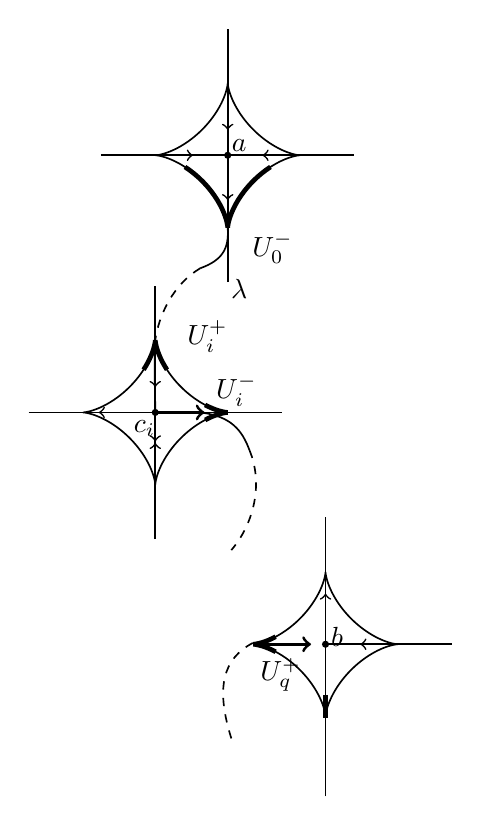
\begin{tikzpicture}[line width=0.6pt,scale=0.92]
  \begin{scope}[shift={(0.4,0)}]
    \draw plot[domain=0:360,samples=181] ({cos(\x)^3},{sin(\x)^3});
    \draw (0,-1.75) -- (0,1.75);
    \draw (-1.75,0) -- (1.75,0);
    \draw[->] (0,0.72) -- (0,0.35);
    \draw[->] (-0.78,0) -- (-0.48,0);
    \draw[->] (0.78,0) -- (0.48,0);
    \draw[line width=1.7pt] plot[domain=213:327,samples=37] ({cos(\x)^3},{sin(\x)^3});
    \fill (0,0) circle (1.4pt);
    \node at (0.16,0.13) {$a$};
    \node at (0.62,-1.28) {$U_0^-$};
    \draw[->] (0,0) -- (0,-0.62);
    \draw (0,-0.5) -- (0,-1.0);
    \draw (0,-1.0) .. controls (0.02,-1.3) and (-0.08,-1.45) .. (-0.38,-1.56);
    \draw[dashed] (-0.38,-1.56) .. controls (-0.75,-1.78) and (-0.95,-2.2) .. (-1.0,-2.55);
    \node at (0.16,-1.85) {$\lambda$};
  \end{scope}
  \begin{scope}[shift={(-0.6,-3.55)}]
    \draw plot[domain=0:360,samples=181] ({cos(\x)^3},{sin(\x)^3});
    \draw (0,-1.75) -- (0,1.75);
    \draw (-1.75,0) -- (1.75,0);
    \draw[->] (0,0.72) -- (0,0.35);
    \draw[->] (0,-0.75) -- (0,-0.42);
    \draw[->] (-0.48,0) -- (-0.78,0);
    \draw[line width=1.7pt] plot[domain=57:123,samples=25] ({cos(\x)^3},{sin(\x)^3});
    \draw[line width=1.7pt] plot[domain=-28:28,samples=21] ({cos(\x)^3},{sin(\x)^3});
    \fill (0,0) circle (1.4pt);
    \node at (-0.15,-0.22) {$c_i$};
    \node at (0.72,1.05) {$U_i^+$};
    \node at (1.12,0.3) {$U_i^-$};
    \draw (0,1.0) .. controls (-0.02,0.6) and (0,0.3) .. (0,0);
    \draw[->] (0,-0.02) -- (0,-0.4);
    \draw[line width=1.1pt] (0,0) -- (0.5,0);
    \draw[line width=1.1pt,->] (0.3,0) -- (0.68,0);
    \draw (0.62,0) .. controls (1.05,-0.05) and (1.2,-0.25) .. (1.3,-0.52);
    \draw[dashed] (1.3,-0.52) .. controls (1.5,-1.0) and (1.35,-1.55) .. (1.05,-1.9);
  \end{scope}
  \begin{scope}[shift={(1.75,-6.75)}]
    \draw plot[domain=0:360,samples=181] ({cos(\x)^3},{sin(\x)^3});
    \draw (0,-2.1) -- (0,1.75);
    \draw (-0.02,0) -- (1.75,0);
    \draw[->] (0,0.35) -- (0,0.7);
    \draw[line width=1.7pt] (0,-0.7) -- (0,-1.02);
    \draw[->] (0.78,0) -- (0.48,0);
    \draw[line width=1.7pt] plot[domain=152:208,samples=21] ({cos(\x)^3},{sin(\x)^3});
    \fill (0,0) circle (1.4pt);
    \node at (0.16,0.1) {$b$};
    \node at (-0.62,-0.42) {$U_q^+$};
    \draw[dashed] (-1.3,-1.3) .. controls (-1.52,-0.6) and (-1.42,-0.2) .. (-1.0,0.02);
    \draw[line width=1.1pt,->] (-0.95,0) -- (-0.2,0);
  \end{scope}
\end{tikzpicture}
\caption{}
\label{fig:broken-neighborhoods}
\end{figure}

我们令 $\mathbf{U}^-$（相应地，$\mathbf{U}^+$）表示诸 $U_i^-$（相应地，诸 $U_i^+$）所成之族，并且我们说 $\mu=(\mu_1,\dotsc,\mu_k)\in\mathcal{W}(\lambda,\mathbf{U}^-,\mathbf{U}^+)$，如果存在整数
\[
0=i_0<i_1<\cdots<i_k=q
\]
使得：
\begin{itemize}
\item 对每个 $1\le j\le k$ 都有 $\mu_j\in\mathcal{L}(c_{i_{j-1}},c_{i_j})$\footnote{译注：原书此处印作 $0<i_0<\cdots<i_{k-1}<i_k=q$，并对每个 $j\le k$ 设 $\mu_j\in\mathcal{L}(c_{i_j},c_{i_{j+1}})$（下列穿图条目亦同用 $i_j$、$i_{j+1}$）；按 $c_0=a$、$c_q=b$（\cref{fig:broken-neighborhoods}）与 $\mu=(\mu_1,\dotsc,\mu_k)$ 的分节，首段应为 $\mathcal{L}(a,c_{i_1})$、末段应为 $\mathcal{L}(c_{i_{k-1}},b)$，而原书首段缺 $a$、且 $j=k$ 时 $i_{k+1}$ 无定义，疑为索引统体错位一位；此处径改为 $0=i_0<i_1<\cdots<i_k=q$、$\mu_j\in\mathcal{L}(c_{i_{j-1}},c_{i_j})$（$j=1,\dotsc,k$），穿图条目随之以 $i_{j-1}$、$i_j$ 记。——译者注}；
\item $\mu_j$ 从相应诸 $U^-$ 的内部穿出诸\trChart{} $\Omega(c_{i_{j-1}})$、$\Omega(c_{i_{j-1}+1})$、……、$\Omega(c_{i_j-1})$，并从诸 $U^+$ 的内部穿入诸\trChart{} $\Omega(c_{i_{j-1}+1})$、……、$\Omega(c_{i_j})$。
\end{itemize}
诸 $\mathcal{W}(\lambda,\mathbf{U}^-,\mathbf{U}^+)$ 构成了 $\overline{\mathcal{L}}(a,b)$ 上一个\trTopology{}的开邻域基本组。

\begin{remark}\label{thm:broken-trajectory-topology}
在这个定义中，$k\le q$（\trTrajectory{} $\mu$ 的分支不会比 $\lambda$ 的多）。此外，如果 $\lambda$ 是 $X$ 的从 $a$ 走到 $b$ 的一条\trTrajectory，那么 $\lambda$ 的一个开邻域基本组就由这样一些连接 $a$ 与 $b$ 的\trTrajectory{}给出：它们离开 $\Omega_0$、进入 $\Omega_q$ 时都充分贴近 $\lambda$。显然，如此得到的\trTopology{}与 $\mathcal{L}(a,b)$ 上的\trTopology{}相重合（后者早已定义为：诸\trTrajectory{}上的点集在平移之下的商）。
\end{remark}

\subsection{\trCompact{}性}
\label{subsec:compactness}

我们现在来证明下述结果。

\begin{theorem}\label{thm:broken-space-compact}
空间 $\overline{\mathcal{L}}(a,b)$ 是\trCompact{}的。
\end{theorem}

\begin{remark}\label{thm:compactness-sequences}
空间 $\overline{\mathcal{L}}(a,b)$ 上的\trTopology{}是利用 $V$ 上的\trTopology{}来定义的。因此，显然它拥有一个可数的开邻域基本组，而用序列来证明\trCompact{}性也就是有理有据的（况且它还是可\trMetric{}化的）。纯粹主义者们还会注意到：我们即将使用的这个空间的\trCompact{}性，说到底也只有序列的这一条性质。
\end{remark}

\begin{corollary}\label{thm:finite-trajectories}
如果 $\operatorname{Ind}(a)=\operatorname{Ind}(b)+1$，那么空间 $\mathcal{L}(a,b)$ 是由\trTrajectory{}构成的一个有限集。
\end{corollary}

于是 $n_X(a,b)\in\ZZ/2$ 是\trWellDefined{}的。这条推论立即可得：此时 $\overline{\mathcal{L}}(a,b)=\mathcal{L}(a,b)$，而后者——它是一个维数为~0 的\trManifold——如今是\trCompact{}的。\noqed

\begin{proof}[\cref{thm:broken-space-compact}的证明]
设 $(\ell_n)$ 是 $\overline{\mathcal{L}}(a,b)$ 中诸\trTrajectory{}的一个序列。

我们先假定 $\ell_n\in\mathcal{L}(a,b)$。\trTrajectory{} $\ell_n$ 通过一点 $\ell_n^-$ 从 $\Omega(a)$ 中穿出，并通过一点 $\ell_n^+$ 进入 $\Omega(b)$。点 $\ell_n^-$ 属于 $a$ 的\trUnstableManifold{}与 $\Omega(a)$ 的边界之交，而后者是一个\trSphere，因而是\trCompact{}的。在必要时抽取一个子序列之后，我们便可以——而且我们也确实——因此假定
\[
\lim\ell_n^-=a^-\qquad\text{并且}\qquad \lim\ell_n^+=b^+\text{。}
\]
设 $\gamma(t)=\varphi_X^t(a^-)$ 是 $a^-$ 的\trTrajectory，并设 $c_1=\lim_{t\to+\infty}\gamma(t)$，于是 $c_1$ 是一个\trCriticalPoint{}，而 $\gamma\in\mathcal{L}(a,c_1)$。设 $d^+$ 是 $\gamma$ 在 $\Omega(c_1)$ 中的入点（\cref{fig:limit-entry-points}）。根据\trDifferential{}方程的解对初始条件的依赖性定理，$\ell_n$ 也必定（至少对充分大的 $n$）进入 $\Omega(c_1)$，入点为 $d_n^+$。由下述引理可知 $\lim d_n^+=d^+$。

\begin{lemma}\label{thm:same-level-convergence}
设 $x\in V-\operatorname{Crit}(f)$，并设 $(x_n)$ 是一个趋于 $x$ 的序列。设 $y_n$ 与 $y$ 分别是位于 $x_n$ 与 $x$ 各自的那条 $X$ 的\trTrajectory{}上的点。我们再假定 $f(y_n)=f(y)$。那么
\[
\lim_{n\to+\infty}y_n=y\text{。}
\]
\end{lemma}

\begin{proof}
设 $U$ 是 $\operatorname{Crit}(f)$ 的一个不包含 $x$、$y$、$x_n$、$y_n$（对充分大的 $n$）的邻域。正如\cref{thm:sublevel-no-critical}的证明中那样，我们考虑\trVectorField
\[
Y=-\frac{1}{df(X)}\cdot X
\]
它定义在 $V-U$ 上。设 $\psi_t$ 表示它的\trFlow。$Y$ 的诸\trTrajectory{}与 $X$ 的相同，而且
\[
f(\psi_t(z))=f(z)-t\text{。}
\]
于是我们有
\[
y_n=\psi_{-f(y_n)+f(x_n)}(x_n)=\psi_{-f(y)+f(x_n)}(x_n)
\]
以及
\[
y=\psi_{-f(y)+f(x)}(x)\text{，}
\]
从而 $\lim y_n=y$。
\end{proof}

\begin{figure}[htbp]
\centering
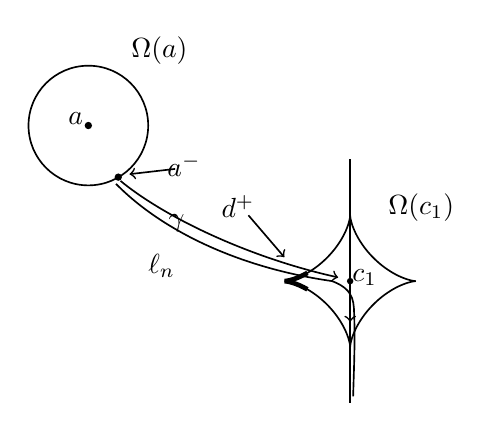
\begin{tikzpicture}[line width=0.6pt,scale=0.95]
  \draw (0,3.2) circle (0.8);
  \fill (0,3.2) circle (1.4pt);
  \node at (-0.17,3.3) {$a$};
  \node at (0.95,4.2) {$\Omega(a)$};
  \fill (0.4,2.51) circle (1.4pt);
  \node at (1.28,2.66) {$a^-$};
  \draw[->] (1.16,2.62) -- (0.55,2.55);
  \draw[->] (0.43,2.46) .. controls (1.05,1.95) and (2.2,1.42) .. (3.34,1.17);
  \draw (0.37,2.42) .. controls (0.98,1.8) and (2.0,1.3) .. (3.26,1.12);
  \draw (3.26,1.12) .. controls (3.44,1.05) and (3.54,0.96) .. (3.55,0.76)
        .. controls (3.57,0.35) and (3.55,-0.05) .. (3.54,-0.42);
  \node at (1.18,1.9) {$\gamma$};
  \node at (0.98,1.32) {$\ell_n$};
  \begin{scope}[shift={(3.5,1.12)},scale=0.88]
    \draw plot[domain=0:360,samples=181] ({cos(\x)^3},{sin(\x)^3});
    \draw (0,-1.85) -- (0,1.85);
    \draw[line width=1.7pt] plot[domain=150:210,samples=21] ({cos(\x)^3},{sin(\x)^3});
    \fill (0,0) circle (1.4pt);
    \node at (0.22,0.06) {$c_1$};
    \draw[->] (0,-0.32) -- (0,-0.62);
    \draw (0,-0.1) -- (0,-1.5);
  \end{scope}
  \node at (4.45,2.1) {$\Omega(c_1)$};
  \node at (2.0,2.12) {$d^+$};
  \draw[->] (2.14,2.0) -- (2.62,1.44);
\end{tikzpicture}
\caption{}
\label{fig:limit-entry-points}
\end{figure}

如果 $c_1=b$，那么我们随之便有 $\lim\ell_n=\gamma$，序列 $\ell_n$ 也就拥有一个\trConvergence{}的子序列。如果情形并非如此，那么 $d_n^+$ 不位于 $c_1$ 的\trStableManifold{}上，从而 $\ell_n$ 通过一点 $d_n^-$ 从 $\Omega(c_1)$ 中穿出。我们可以——而且我们也确实——假定序列 $d_n^-$ \trConvergence{}于一点 $d^-$。这个点位于 $c_1$ 的\trUnstableManifold{}之上。倘若不是这样，那么 $d^-$ 就会位于 $d_{\star}$ 的某条\trTrajectory{}之上，其中 $f(d_{\star})=f(d_n^+)$，而且这条\trTrajectory{}还不属于 $W^s(c_1)$。由前一条引理，$d_n^+$ 趋于 $d_{\star}$，于是 $d_{\star}=d^+$，而这是荒谬的，因为 $d^+\in W^s(c_1)$。

剩下的就是考虑 $\overline{\mathcal{L}}(a,b)$ 中元素之序列的一般情形。存在\trCriticalPoint{} $c_1,\dotsc,c_{q-1}$，使得对充分大的 $n$，在抽取一个子序列之后，我们有
\[
\ell_n=(\ell_n^1,\dotsc,\ell_n^q)\in\mathcal{L}(a,c_1)\times\cdots\times\mathcal{L}(c_{q-1},b)\text{。}
\]
我们把前面的结果应用于 $\ell_n^1$，随后再应用于 $\ell_n^2,\dotsc,\ell_n^q$。
\end{proof}

请注意，正如记号所提示的那样，$\overline{\mathcal{L}}(a,b)$ 确实是 $\mathcal{L}(a,b)$ 的一个\trCompactification，其含义是：对 $\overline{\mathcal{L}}(a,b)$ 的任一元素，$\mathcal{L}(a,b)$ 中都存在任意贴近它的元素。这是下述命题的一个推论，而该命题本身又是\cref{thm:broken-space-compact}的证明中所用诸论证（也就是说，\trCauchy--\trLipschitz{}定理的论证）的一个推论。

\begin{proposition}\label{thm:approximate-broken}
设 $\lambda=(\lambda_1,\lambda_2)\in\overline{\mathcal{L}}(a,b)$，其中 $\lambda_1\in\mathcal{L}(a,c)$、$\lambda_2\in\mathcal{L}(c,b)$。对每一对 $\mathbf{U}^-$、$\mathbf{U}^+$，都存在一个
\[
\ell\in\mathcal{L}(a,b)\cap\mathcal{W}(\lambda,\mathbf{U}^-,\mathbf{U}^+)\text{。}
\]
\noqed
\end{proposition}

在下一小节中，我们将对这个命题给出更多的细节。

\subsection{\trBrokenTrajectory{}空间上的\trManifoldWithBoundary{}结构}
\label{subsec:manifold-structure-broken}

下述定理蕴含着 $\partial_X\circ\partial_X=0$。

\begin{theorem}\label{thm:broken-manifold-boundary}
如果 $\operatorname{Ind}(a)=\operatorname{Ind}(b)+2$，那么 $\overline{\mathcal{L}}(a,b)$ 是一个维数为~1 的\trCompact{}\trManifoldWithBoundary。
\end{theorem}

我们已经知道 $\mathcal{L}(a,b)$ 是一个维数为~1 的\trManifold（通过应用\trSmaleCondition）。因此，该定理是下述命题的一个推论。

\begin{proposition}\label{thm:gluing-embedding}
设 $V$ 是一个\trCompact\trManifold，设 $f\colon V\to\RR$ 是一个\trMorseFunction，并设 $X$ 是 $f$ 的一个满足\trSmale{}性质的\trPseudogradient。设 $a$、$c$ 与 $b$ 是\trIndex{}分别为 $k+1$、$k$ 与 $k-1$ 的三个\trCriticalPoint。设 $\lambda_1\in\mathcal{L}(a,c)$ 与 $\lambda_2\in\mathcal{L}(c,b)$。那么存在一个连续\trEmbedding{} $\psi$，它把一个区间 $[0,\delta[$ 映满到 $(\lambda_1,\lambda_2)$ 在 $\overline{\mathcal{L}}(a,b)$ 中的一个邻域上，它在 $[0,\delta[$ 上可微，并且满足
\[
\begin{cases}
\psi(0)=(\lambda_1,\lambda_2)\in\overline{\mathcal{L}}(a,b)\\
\psi(s)\in\mathcal{L}(a,b) & \text{对 } s\neq 0\text{。}
\end{cases}
\]
此外，如果 $(\ell_n)$ 是 $\mathcal{L}(a,b)$ 中趋于 $(\lambda_1,\lambda_2)$ 的一个序列，那么对充分大的 $n$，$\ell_n$ 都包含在 $\psi$ 的像之中。
\end{proposition}

\begin{remark}\label{thm:single-branch}
最后这条断言，对于证明 $(\lambda_1,\lambda_2)$ 是边界上的一点而言是必不可少的：到达那里的分支只有一支。
\end{remark}

\begin{figure}[htbp]
\centering
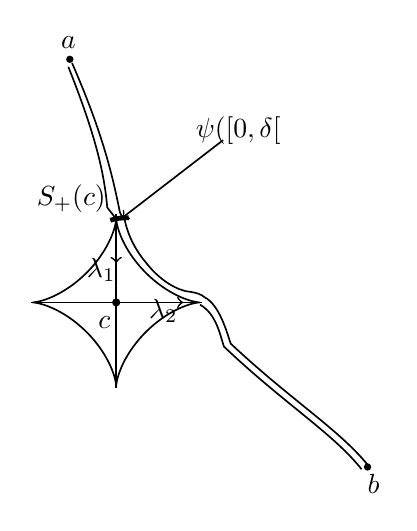
\begin{tikzpicture}[line width=0.6pt,scale=0.95]
  \fill (0,5.0) circle (1.4pt);
  \node at (-0.02,5.22) {$a$};
  \draw (0.03,4.95) .. controls (0.4,4.1) and (0.55,3.55) .. (0.66,3.0)
        .. controls (0.67,2.92) and (0.70,2.90) .. (0.73,2.87)
        .. controls (0.78,2.62) and (0.90,2.42) .. (1.02,2.28)
        .. controls (1.16,2.10) and (1.35,1.95) .. (1.55,1.90)
        .. controls (1.68,1.885) and (1.76,1.86) .. (1.80,1.82);
  \draw (-0.02,4.9) .. controls (0.33,4.02) and (0.46,3.5) .. (0.50,3.02)
        .. controls (0.56,2.94) and (0.60,2.90) .. (0.605,2.875);
  \node at (2.25,4.05) {$\psi([0,\delta[$};
  \draw[->] (2.05,3.92) -- (0.70,2.88);
  \begin{scope}[shift={(0.62,1.75)},scale=1.12]
    \draw plot[domain=0:360,samples=181] ({cos(\x)^3},{sin(\x)^3});
    \draw (0,-1.02) -- (0,1.05);
    \draw (-1.02,0) -- (1.02,0);
    \draw[->] (0,0.68) -- (0,0.47);
    \draw[->] (0.45,0) -- (0.8,0);
    \draw[line width=1.7pt] (-0.07,0.98) .. controls (-0.02,1.0) and (0.06,1.01) .. (0.15,1.01);
    \fill (0,0) circle (1.4pt);
    \node at (-0.14,-0.24) {$c$};
  \end{scope}
  \node at (0.02,3.14) {$S_+(c)$};
  \node at (0.42,2.18) {$\lambda_1$};
  \node at (1.25,1.64) {$\lambda_2$};
  \draw (1.80,1.82) .. controls (2.00,1.72) and (2.10,1.35) .. (2.15,1.20)
        .. controls (2.95,0.45) and (3.6,0.05) .. (3.98,-0.42);
  \draw (1.74,1.72) .. controls (1.95,1.60) and (2.00,1.35) .. (2.06,1.16)
        .. controls (2.86,0.4) and (3.52,0.0) .. (3.9,-0.48);
  \fill (3.98,-0.45) circle (1.4pt);
  \node at (4.06,-0.68) {$b$};
\end{tikzpicture}
\caption{}
\label{fig:gluing-family}
\end{figure}

\begin{proof}[\cref{thm:gluing-embedding}的证明]
我们令 $f(c)=\alpha$，并选取 $\varepsilon>0$，使得 $f^{-1}(\alpha+\varepsilon)$ 与 $f^{-1}(\alpha-\varepsilon)$ 分别沿着 $\partial_+\Omega(c)$ 与 $\partial_-\Omega(c)$ 与\trMorseChart{} $\Omega(c)$ 相交。我们采用前面定义的记号，即
\[
\begin{aligned}
S_+(c)&=W^s(c)\cap f^{-1}(\alpha+\varepsilon)\cong S^{n-k-1}\\
S_-(c)&=W^u(c)\cap f^{-1}(\alpha-\varepsilon)\cong S^{k-1}\text{。}
\end{aligned}
\]
设 $a_1=S_+(c)\cap\lambda_1$。\trUnstableManifold{} $W^u(a)$ 沿着一个维数为 $k$ 的\trSubmanifold{} $P$ \trTransverse{}地遇到 $f^{-1}(\alpha+\varepsilon)$。由于 $X$ 满足\trSmale{}性质，$P$ 与 $S_+(c)$ \trTransverse{}地相交于有限多个点，其中包括点 $a_1$。设
\[
D^k(\delta)=\{(x_1,\dotsc,x_k) \mid \|x\|<\delta\}
\]
并设 $\Psi\colon(D^k(\delta),0)\to(P,a_1)$ 是 $P$ 的一个局部\trParametrization，使得
\[
\operatorname{Im}\Psi\cap S_+(c)=\{a_1\}\text{。}
\]
我们可以——而且我们也确实——假定 $D=\operatorname{Im}\Psi$ 包含在 $\partial_+\Omega(c)$ 之中。\trDisk{} $D$ 在\cref{fig:disk-descent}中被画成阴影。让 $D-\{a_1\}$ 沿着 $X$ 的诸\trTrajectory{}下降，我们便得到一个\trEmbedding
\[
\Phi\colon D-\{a_1\}\longrightarrow\partial_-\Omega(c)\text{。}
\]

\begin{figure}[htbp]
\centering
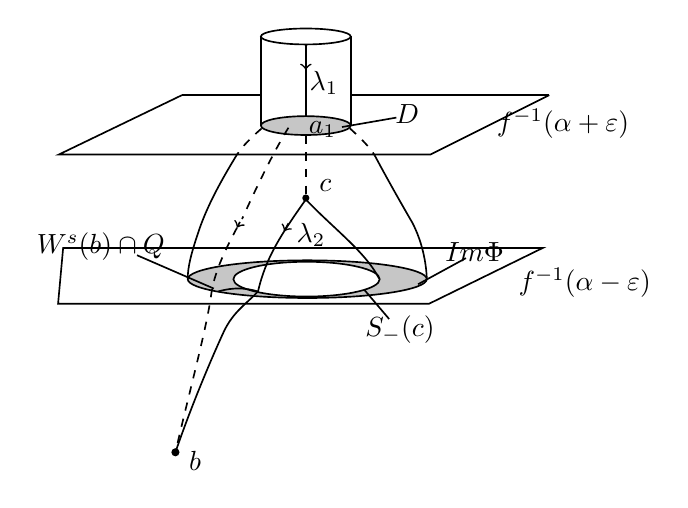
\begin{tikzpicture}[line width=0.6pt,scale=0.92]
  \draw (-1.66,4.61) -- (-0.57,4.61);
  \draw (0.67,4.61) -- (3.41,4.61);
  \draw (-1.66,4.61) -- (-3.36,3.79) -- (1.77,3.79) -- (3.41,4.61);
  \node at (3.60,4.22) {$f^{-1}(\alpha+\varepsilon)$};
  \draw (-3.30,2.50) -- (3.32,2.50) -- (1.75,1.73) -- (-3.37,1.73) -- cycle;
  \node at (3.90,2.02) {$f^{-1}(\alpha-\varepsilon)$};
  \draw (-0.57,4.19) -- (-0.57,5.42);
  \draw (0.67,4.19) -- (0.67,5.42);
  \draw (0.05,5.42) ellipse (0.62 and 0.11);
  \fill[gray!45] (0.05,4.19) ellipse (0.62 and 0.13);
  \draw (0.05,4.19) ellipse (0.62 and 0.13);
  \node at (0.28,4.13) {$a_1$};
  \node at (1.45,4.35) {$D$};
  \draw (1.30,4.30) -- (0.55,4.17);
  \draw (0.05,5.31) -- (0.05,4.32);
  \draw[->] (0.05,5.12) -- (0.05,4.96);
  \node at (0.30,4.78) {$\lambda_1$};
  \draw[dashed] (0.05,4.05) -- (0.05,3.23);
  \fill[even odd rule,gray!45] (0.07,2.07) ellipse (1.65 and 0.26)
    (0.06,2.07) ellipse (1.01 and 0.24);
  \draw (0.07,2.07) ellipse (1.65 and 0.26);
  \draw (0.06,2.07) ellipse (1.01 and 0.24);
  \draw[dashed] (-0.56,4.15) .. controls (-0.70,4.03) and (-0.82,3.91) .. (-0.90,3.79);
  \draw (-0.90,3.79) .. controls (-1.12,3.43) and (-1.32,3.07) .. (-1.44,2.70)
        .. controls (-1.53,2.43) and (-1.58,2.24) .. (-1.58,2.08);
  \draw[dashed] (0.66,4.15) .. controls (0.79,4.03) and (0.92,3.91) .. (1.00,3.78);
  \draw (1.00,3.78) .. controls (1.16,3.48) and (1.34,3.16) .. (1.52,2.85)
        .. controls (1.65,2.60) and (1.71,2.32) .. (1.72,2.08);
  \draw (0.05,3.17) .. controls (0.42,2.78) and (0.88,2.44) .. (1.06,2.08);
  \draw (0.05,3.17) .. controls (-0.28,2.70) and (-0.50,2.38) .. (-0.61,1.90)
        .. controls (-0.78,1.72) and (-0.95,1.62) .. (-1.08,1.35)
        .. controls (-1.25,0.98) and (-1.52,0.35) .. (-1.75,-0.32);
  \draw[->] (-0.19,2.84) -- (-0.25,2.73);
  \node at (0.12,2.68) {$\lambda_2$};
  \fill (0.05,3.19) circle (1.4pt);
  \node at (0.32,3.36) {$c$};
  \draw[dashed] (-0.19,4.16) .. controls (-0.40,3.82) and (-0.65,3.30) .. (-0.83,2.90);
  \draw[dashed,->] (-0.86,2.86) -- (-0.90,2.78);
  \draw[dashed] (-0.90,2.78) .. controls (-1.08,2.44) and (-1.22,2.15) .. (-1.26,1.83)
        .. controls (-1.33,1.35) and (-1.55,0.55) .. (-1.75,-0.32);
  \draw (-1.16,1.90) .. controls (-0.95,1.96) and (-0.78,1.95) .. (-0.61,1.90);
  \node at (-2.78,2.52) {$W^s(b)\cap Q$};
  \draw (-2.28,2.40) -- (-1.22,1.94);
  \node at (2.38,2.44) {$\operatorname{Im}\Phi$};
  \draw (2.26,2.36) -- (1.60,2.00);
  \node at (1.35,1.38) {$S_-(c)$};
  \draw (1.20,1.52) -- (0.86,1.92);
  \fill (-1.75,-0.32) circle (1.6pt);
  \node at (-1.48,-0.44) {$b$};
\end{tikzpicture}
\caption{}
\label{fig:disk-descent}
\end{figure}

$\Phi$ 的像就是\cref{fig:disk-descent}中所示的那个带阴影的圆环\footnote{这幅图正是整个证明的要害。}（在这幅图中，$S_-(c)$ 是带阴影圆环的内边界）。我们有下述结果。

\begin{proposition}\label{thm:annulus-boundary}
在必要时先限制 $D$ 的大小——也就是说，必要时先把 $\Psi$ 限制到一个半径 $\delta'<\delta$ 的\trDisk{}上——则并集
$Q=\operatorname{Im}\Phi\cup S_-(c)$
是一个维数为 $k$ 的\trManifoldWithBoundary，而它的边界为 $\partial Q=S_-(c)$。
\end{proposition}

这条命题使我们得以结束\cref{thm:gluing-embedding}的证明。$\Phi$ 的像是 $a$ 的\trUnstableManifold{}与\trLevelSet{} $f^{-1}(\alpha-\varepsilon)$ 之交中的一个\trOpen{}子集。由于 $X$ 具有\trSmale{}性质，我们随即便有
\[
W^s(b)\pitchfork\operatorname{Im}\Phi
\]
而且我们也有
\[
W^s(b)\pitchfork S_-(c)\text{。}
\]
从而 $W^s(b)\cap Q$ 将是 $\partial_-\Omega(c)\subset f^{-1}(\alpha-\varepsilon)$ 中一个维数为~1 的\trSubmanifold，而它的边界是 $W^s(b)\cap\partial Q=\mathcal{L}(c,b)$。

设 $a_2$ 是 $\lambda_2$ 与 $S_-(c)$ 的交点，并让我们定义一个\trParametrization
\[
\chi\colon[0,\delta[\,\longrightarrow W^s(b)\cap Q
\]
把这个\trManifoldWithBoundary{}\trParametrization：点 $0$ 被送到点 $a_2$。我们还有一个映射
\[
\Phi^{-1}\circ\chi\colon\,]0,\delta[\,\longrightarrow W^s(b)\cap(D-\{a_1\})\text{。}
\]
当 $s\to 0$ 时，值 $\Phi^{-1}\circ\chi(s)$ 趋于 $a_1$（通过应用\cref{thm:same-level-convergence}）。因此我们可以把它延拓到 $[0,\delta[$ 上，从而得到所想要的 $\psi$：
\[
\psi\colon[0,\eta[\,\longrightarrow\overline{\mathcal{L}}(a,b)
\qquad\text{其中 }\psi(0)=(\lambda_1,\lambda_2)\text{。}
\]
现在，设 $(\ell_n)$ 是 $\mathcal{L}(a,b)$ 中趋于 $(\lambda_1,\lambda_2)$ 的一个序列。设 $\ell_n^+$ 与 $\ell_n^-$ 表示 $\ell_n$ 在 $c$ 的\trMorseChart{}中的入点与出点。我们有
\[
\lim_{n\to+\infty}\ell_n^+=a_1\text{，}\quad
\lim_{n\to+\infty}\ell_n^-=a_2
\quad\text{以及}\quad \Phi(\ell_n^+)=\ell_n^-\text{。}
\]
对充分大的 $n$，$\ell_n^+\in D-\{a_1\}$，从而 $\ell_n^-\in Q$，这就蕴含着
\[
\ell_n^-\in Q\cap W^s(b)=\operatorname{Im}\chi\text{。}
\]
由此可知 $\ell_n\in\operatorname{Im}\psi$。
\end{proof}

我们还须证明这条命题。让我们先把它在\trMorse{}模型 $U\subset\RR^k\times\RR^{n-k}$ 中重新陈述一遍，其中
\[
f(x_-,x_+)=-\|x_-\|^2+\|x_+\|^2\text{，}\qquad X=-\operatorname{grad}f
\]
以及
\[
\begin{aligned}
S_+&=\{(x_-,x_+)\mid x_-=0,\ \|x_+\|^2=\varepsilon\}\subset f^{-1}(\varepsilon)\text{，}\\
S_-&=\{(x_-,x_+)\mid x_+=0,\ \|x_-\|^2=\varepsilon\}\subset f^{-1}(-\varepsilon)\text{。}
\end{aligned}
\]

\begin{figure}[htbp]
\centering
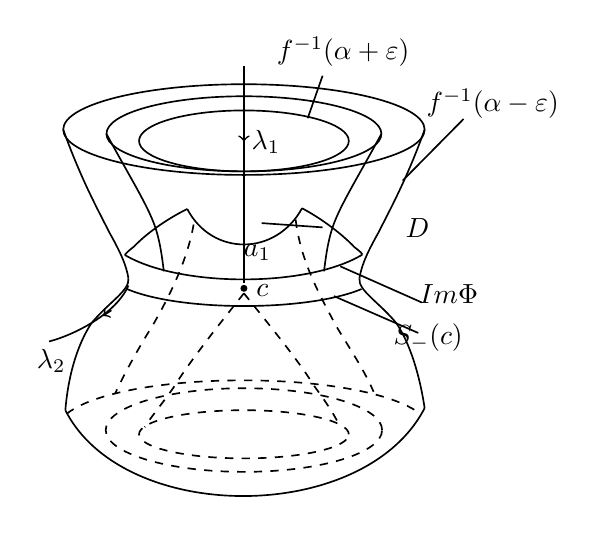
\begin{tikzpicture}[line width=0.6pt,scale=0.9]
  \draw (0,2.15) ellipse (2.55 and 0.64);
  \draw (0,2.09) ellipse (1.94 and 0.53);
  \draw (0,1.99) ellipse (1.48 and 0.43);
  \draw (-2.55,2.15) .. controls (-2.30,1.45) and (-2.05,1.00) .. (-1.90,0.70)
        .. controls (-1.76,0.45) and (-1.66,0.25) .. (-1.63,0.05);
  \draw (2.55,2.15) .. controls (2.30,1.45) and (2.05,1.00) .. (1.90,0.70)
        .. controls (1.76,0.45) and (1.66,0.25) .. (1.63,0.05);
  \draw (-1.63,0.05) .. controls (-1.61,-0.12) and (-1.90,-0.28) .. (-2.15,-0.58)
        .. controls (-2.35,-0.88) and (-2.48,-1.32) .. (-2.52,-1.81);
  \draw (1.63,0.05) .. controls (1.61,-0.12) and (1.90,-0.28) .. (2.15,-0.58)
        .. controls (2.35,-0.88) and (2.48,-1.32) .. (2.55,-1.78);
  \draw (-1.94,2.09) .. controls (-1.62,1.50) and (-1.40,1.15) .. (-1.28,0.85)
        .. controls (-1.18,0.60) and (-1.15,0.30) .. (-1.13,0.15);
  \draw (1.94,2.09) .. controls (1.62,1.50) and (1.40,1.15) .. (1.28,0.85)
        .. controls (1.18,0.60) and (1.15,0.30) .. (1.13,0.15);
  \draw (-1.68,0.38) .. controls (-0.90,-0.08) and (0.90,-0.08) .. (1.67,0.385);
  \draw (-1.65,-0.10) .. controls (-0.90,-0.42) and (0.90,-0.42) .. (1.66,-0.10);
  \draw (-2.52,-1.81) .. controls (-1.70,-3.43) and (1.70,-3.43) .. (2.55,-1.78);
  \draw[dashed] (-2.50,-1.86) .. controls (-1.70,-1.23) and (1.70,-1.23) .. (2.50,-1.87);
  \draw[dashed] (0,-2.09) ellipse (1.95 and 0.59);
  \draw[dashed] (0,-2.15) ellipse (1.48 and 0.34);
  \draw (-0.80,1.03) .. controls (-0.45,0.36) and (0.45,0.36) .. (0.82,1.04);
  \draw (-0.80,1.03) .. controls (-1.10,0.88) and (-1.38,0.68) .. (-1.55,0.50)
        .. controls (-1.63,0.44) and (-1.67,0.40) .. (-1.68,0.38);
  \draw (0.82,1.04) .. controls (1.12,0.88) and (1.40,0.66) .. (1.56,0.49)
        .. controls (1.64,0.43) and (1.67,0.40) .. (1.67,0.385);
  \draw (0,3.05) -- (0,-0.02);
  \draw[->] (0,2.16) -- (0,1.98);
  \node at (0.31,1.98) {$\lambda_1$};
  \node at (0.19,0.41) {$a_1$};
  \fill (0,-0.09) circle (1.4pt);
  \node at (0.26,-0.12) {$c$};
  \draw[dashed] (0,-0.16) .. controls (-0.35,-0.60) and (-0.75,-1.10) .. (-1.00,-1.50)
        .. controls (-1.20,-1.78) and (-1.33,-1.93) .. (-1.40,-2.05);
  \draw[dashed] (0,-0.16) .. controls (0.35,-0.60) and (0.75,-1.08) .. (1.00,-1.48)
        .. controls (1.20,-1.75) and (1.32,-1.95) .. (1.36,-2.06);
  \draw[dashed] (-0.71,0.81) .. controls (-0.80,0.30) and (-1.05,-0.20) .. (-1.28,-0.60)
        .. controls (-1.48,-0.92) and (-1.68,-1.28) .. (-1.82,-1.58);
  \draw[dashed] (0.73,0.88) .. controls (0.80,0.28) and (1.08,-0.20) .. (1.30,-0.62)
        .. controls (1.50,-0.95) and (1.70,-1.25) .. (1.83,-1.55);
  \draw (-1.63,-0.05) .. controls (-1.80,-0.45) and (-2.40,-0.75) .. (-2.75,-0.84);
  \draw[->] (-1.87,-0.40) -- (-1.99,-0.48);
  \node at (-2.72,-1.12) {$\lambda_2$};
  \node at (1.40,3.25) {$f^{-1}(\alpha+\varepsilon)$};
  \draw (1.11,2.91) -- (0.90,2.31);
  \node at (3.51,2.51) {$f^{-1}(\alpha-\varepsilon)$};
  \draw (3.10,2.30) -- (2.24,1.43);
  \node at (2.45,0.76) {$D$};
  \draw (1.11,0.77) -- (0.25,0.83);
  \node at (2.89,-0.17) {$\operatorname{Im}\Phi$};
  \draw (2.51,-0.29) -- (1.36,0.22);
  \node at (2.60,-0.79) {$S_-(c)$};
  \draw (2.46,-0.72) -- (1.27,-0.20);
\end{tikzpicture}
\caption{}
\label{fig:morse-model-descent}
\end{figure}

\cref{fig:morse-model-descent}所示的内容与\cref{fig:disk-descent}完全相同，只是如今处在\trMorseChart{}之中（$f$ 的诸\trLevelSet{}不再由一些水平平面来表现，而是由一些\trQuadric{}来表现）。

\begin{proposition}\label{thm:morse-model-annulus}
设 $a\in S_+$，并设 $D\subset\partial_+U$ 是一个维数为 $k$、半径为 $\delta$ 的\trDisk，它与 $S_+$ \trTransverse{}地相交于 $a$。设
\[
\Phi\colon\partial_+U-S_+\longrightarrow\partial_-U-S_-
\]
是由 $X$ 的\trFlow{}所定义的\trEmbedding。那么
\[
Q=\Phi(D-\{a\})\cup S_-
\]
是一个\trManifoldWithBoundary，而它的边界为 $\partial Q=S_-$。
\end{proposition}

为了证明这条命题，我们还要再用到一条引理。

\begin{lemma}\label{thm:embedding-formula}
由 $X$ 的\trFlow{}所定义的\trEmbedding
\[
\Phi\colon\partial_+U-S_+\longrightarrow\partial_-U-S_-
\]
由下式给出：
\[
\Phi(x_-,x_+)=\Bigl(\frac{\|x_+\|}{\|x_-\|}\,x_-,
  \frac{\|x_-\|}{\|x_+\|}\,x_+\Bigr)\text{。}
\]
\end{lemma}

\begin{proof}
我们只需积分 $X$，它的\trFlow{}是
\[
\varphi^s(x_-,x_+)=(e^{2s}x_-,e^{-2s}x_+)\text{。}
\]
如果 $(x_-,x_+)\in\partial_+U$ 且 $x_-\neq 0$，那么存在一个 $s$ 使得
\[
\Bigl(\frac{\|x_+\|}{\|x_-\|}\,x_-,
  \frac{\|x_-\|}{\|x_+\|}\,x_+\Bigr)=(e^{2s}x_-,e^{-2s}x_+)\text{。}
\]
由于 $\|x_+\|>\|x_-\|$，我们有 $s>0$；此外，
\[
\Bigl(\frac{\|x_+\|}{\|x_-\|}\,x_-,
  \frac{\|x_-\|}{\|x_+\|}\,x_+\Bigr)\in\partial_-U\text{。}\qedhere
\]
\end{proof}

\begin{proof}[\cref{thm:annulus-boundary}或\cref{thm:morse-model-annulus}的证明]
设 $D$ 是\cref{thm:morse-model-annulus}的陈述中的那类\trDisk。由于 $S_+$ 由那些满足 $x_-=0$ 的 $x$ 组成，并且 $D\pitchfork S_+$，我们知道 $0$ 是投影
\[
\pi\colon\partial_+U\longrightarrow D^k\text{，}\qquad \pi(x_-,x_+)=x_-
\]
限制到 $D$ 上的一个\trRegularValue。利用\trLocalInversionTheorem，我们可以——而且我们也确实——假定
\[
D=\{(x_-,h(x_-)) \mid x_-\in D^k(\delta)\}
\]
其中 $h\colon D^k(\delta)\to D^{n-k}$ 满足
\[
\|h(x_-)\|^2=\|x_-\|^2+\varepsilon\text{，}
\qquad\text{也就是说，}(x_-,h(x_-))\in\partial_+U\text{。}
\]
我们令 $g=h/\|h\|\colon D^k\to S^{n-k-1}$，于是
\[
D=\bigl\{(x_-, \sqrt{\varepsilon+\|x_-\|^2}\,g(x_-)) \bigm| x_-\in D^k(\delta)\bigr\}\text{。}
\]
由这条引理，我们有
\[
\Phi(D-\{a\})=\Bigl\{\bigl(\sqrt{\varepsilon+\|x_-\|^2}\,x_-/\|x_-\|,
  \|x_-\|\,g(x_-)\bigr) \Bigm| x_-\in D^k(\delta)-\{0\}\Bigr\}\text{。}
\]
让我们在 $D^k(\delta)-\{0\}$ 上使用“极”坐标 $(\rho,u)\in\left]0,\delta\right[\,\times S^{k-1}$。于是 $\Phi(D-\{a\})$ 就是
\[
\begin{aligned}
H\colon\left]0,\delta\right[\,\times S^{k-1} &\longrightarrow \partial_-U\\
(\rho,u) &\longmapsto \bigl(\sqrt{\rho^2+\varepsilon}\,u,\ \rho g(\rho,u)\bigr)
\end{aligned}
\]
的像。由于映射 $g$ 定义在整个\trDisk{} $D^k$ 上，我们可以通过令
\[
H(0,u)=(\sqrt{\varepsilon}\,u,0)\in S_-
\]
而把 $H$ 延拓到乘积 $[0,\delta]\times S^{k-1}$ 上。从而，$\Phi(D-\{a\})\cup S_-$ 确实是一个\trManifoldWithBoundary，而它的边界是 $S_-$。
\end{proof}

\emph{结论。}

我们如今已经证明了本节开头所预告的事情：两个\trCriticalPoint{}之间的诸连接所成之集，可以通过添加诸\trBrokenTrajectory{}来\trCompactification。

\subsection{\trManifoldWithBoundary}
\label{subsec:manifolds-with-boundary}

$C_{\star}(f)$ 的构造、$\partial_X$ 的定义以及 $\partial_X\circ\partial_X=0$ 这个事实，都可以推广到\trManifoldWithBoundary{}的情形，只要 $f$ 的诸\trCriticalPoint{}都不位于边界之上，并且场 $X$ 与这个边界\trTransverse{}（不相切），从而诸\trCriticalPoint{}之间的诸连接都远离边界。更一般的讨论，参见\cref{subsec:morse-functions-adapted-fields}与\cref{sec:cobordisms}。

\begin{remark}\label{thm:cornered-boundary}
对于一个\textbf{\trCorneredBoundary\trManifold}（manifold with cornered boundary）\footnote{我们采用这个术语，来翻译 François~Latour~[46] 为 “with boundary and corners”（带角与边）所引入的雅词 “variété à bord anguleux”（法语，意为“带角的边界\trManifold”）。}$V\times[0,1]^k$，我们将会需要一个类似的定义。我们要求：在边界 $\partial(V\times[0,1]^k)$ 的附近，\trPseudogradient{}具有如下形状：
\[
Y+g_1(t_1)\frac{\partial}{\partial t_1}+\cdots+g_k(t_k)\frac{\partial}{\partial t_k}
\]
其中 $Y$ 是一个在 $V$ 的边界附近与 $X$ 相重合的\trVectorField，而诸函数 $g_i$ 在 $0$ 与 $1$ 处都非零。
\end{remark}
